\section{Preventivo}
Questa sezione contiene un preventivo del costo del lavoro da svolgere dai membri di \groupName{} in modo da definire il budget del progetto. \newline
Le seguenti sigle saranno utilizzate per identificare i vari ruoli:
    \begin{itemize}
        \item Re: \roleProjectManager;
        \item Am: \roleAdministrator;
        \item An: \roleAnalyst;
        \item Pt: \roleDesigner;
        \item Pr: \roleProgrammer;
        \item Ve: \roleVerifier.
    \end{itemize}

    \subsection{Fase di analisi}
    Le ore di lavoro in questa fase sono da considerare come investimento da parte di \groupName{} e non saranno rendicontate nel budget richiesto.
    Vengono rese disponibili in quanto utili ai fini del documento. 
        \subsubsection{Prospetto orario}
        In questa fase, ogni membro del \groupName{} ricoprirà i seguenti ruoli:
        \begin{table}[H]
            
            \centering
            \renewcommand{\arraystretch}{2.6}
            \rowcolors{3}{tableRow}{}
            \begin{tabular}{c c c c c c c c}
                \rowcolor[HTML]{232f3e} 
                \multicolumn{1}{c}{\color[HTML]{FFFFFF} \textbf{Nominativo}} &
                \multicolumn{1}{c}{\color[HTML]{FFFFFF} \textbf{Re}} &
                \multicolumn{1}{c}{\color[HTML]{FFFFFF} \textbf{Am}} &
                \multicolumn{1}{c}{\color[HTML]{FFFFFF} \textbf{An}} &
                \multicolumn{1}{c}{\color[HTML]{FFFFFF} \textbf{Pt}} &
                \multicolumn{1}{c}{\color[HTML]{FFFFFF} \textbf{Pr}} &
                \multicolumn{1}{c}{\color[HTML]{FFFFFF} \textbf{Ve}} &
                \multicolumn{1}{c}{\color[HTML]{FFFFFF} \textbf{Totale}} \\
                \andrea &8&5&12&-&-&-&25\\ 
                \daniele &5&10&5&-&-&5&25\\
                \davide &-&-&4&6&-&15&25\\
                \valentin &5&-&6&6&-&8&25\\
                \giacomo &-&5&15&5&-&-&25\\
                \francesco &5&-&15&-&-&5&25\\ 
                \singh &-&5&15&-&-&5&25\\
            \end{tabular}
            \caption {Distribuzione di ore nella fase di analisi} \label{table:Suddivisione ruoli in ore}
        \end{table}

        \pagebreak

        È possibile raffigurare l'allocazione dei ruoli nel seguente istogramma:
        \begin{figure}[H]
            \centering
            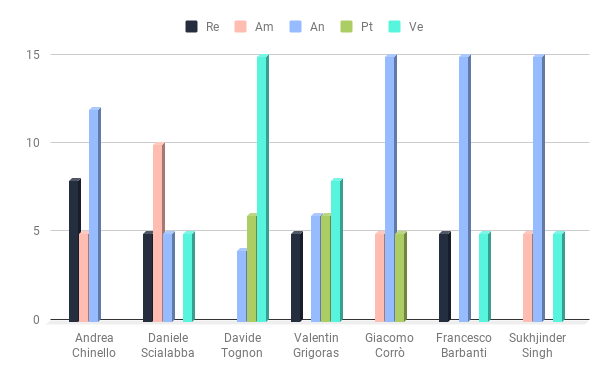
\includegraphics[scale=0.6]{immagini/analisi_isto.png}
            \caption{Istogramma della distribuzione delle ore per ruolo in fase di \textit{Analisi}}
        \end{figure}

        \subsubsection{Prospetto economico}
        Le ore e i costi dei vari ruoli di questa fase sono i seguenti:
        \begin{table}[H]
            
            \centering
            \renewcommand{\arraystretch}{2.6}
            \rowcolors{3}{tableRow}{}
            \begin{tabular}{c c c}
                \rowcolor[HTML]{232f3e} 
                \multicolumn{1}{c}{\color[HTML]{FFFFFF} \textbf{Ruolo}} &
                \multicolumn{1}{c}{\color[HTML]{FFFFFF} \textbf{Ore}} &
                \multicolumn{1}{c}{\color[HTML]{FFFFFF} \textbf{Costo}} \\
                \roleProjectManager&23&690,00 \euro\\
                \roleAdministrator&25&500,00\\
                \roleAnalyst&72&1800,00 \euro\\
                \roleDesigner&17&374,00 \euro\\
                \roleProgrammer&0&0\\
                \roleVerifier&38&570,00 \euro\\
                \textbf{Totale}&\textbf{175}&\textbf{3934,00 \euro}\\
            \end{tabular}
            \caption {Ore e costo per ruolo durante la fase di analisi} \label{table:Prospetto economico tabella}
        \end{table} 
        
        \pagebreak

        La suddivisione dei ruoli è così riassumibile:
        \begin{figure}[H]
            \centering
            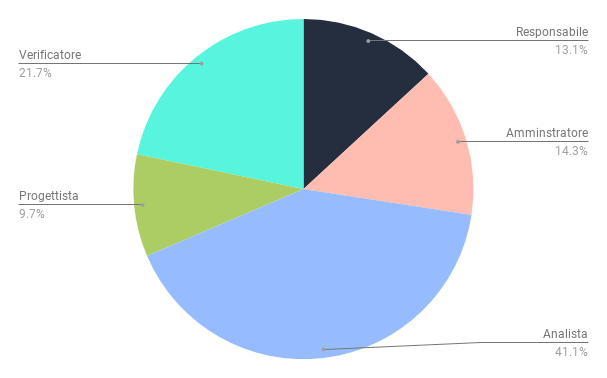
\includegraphics[scale=0.6]{immagini/analisi_pie.png}
            \caption{Aerogramma della distribuzione delle ore per ruolo in fase di analisi}
        \end{figure}

    \subsection{Fase di progettazione architetturale}
        \subsubsection{Prospetto orario}
            La distribuzione oraria di questa fase è la seguente:
        \begin{table}[H]
            
            \centering
            \renewcommand{\arraystretch}{2.6}
            \rowcolors{3}{tableRow}{}
            \begin{tabular}{c c c c c c c c}
                \rowcolor[HTML]{232f3e} 
                \multicolumn{1}{c}{\color[HTML]{FFFFFF} \textbf{Nominativo}} &
                \multicolumn{1}{c}{\color[HTML]{FFFFFF} \textbf{Re}} &
                \multicolumn{1}{c}{\color[HTML]{FFFFFF} \textbf{Am}} &
                \multicolumn{1}{c}{\color[HTML]{FFFFFF} \textbf{An}} &
                \multicolumn{1}{c}{\color[HTML]{FFFFFF} \textbf{Pt}} &
                \multicolumn{1}{c}{\color[HTML]{FFFFFF} \textbf{Pr}} &
                \multicolumn{1}{c}{\color[HTML]{FFFFFF} \textbf{Ve}} &
                \multicolumn{1}{c}{\color[HTML]{FFFFFF} \textbf{Totale}} \\
                \andrea &-&-&-&5&9&13&27\\
                \daniele &-&-&-&13&5&9&27\\
                \davide &-&-&-&11&9&7&27\\
                \valentin &5&-&-&8&6&8&27\\
                \giacomo &7&-&9&-&6&5&27\\
                \francesco &-&4&-&-&9&14&27\\ 
                \singh &-&4&9&-&5&9&27\\
            \end{tabular}
            \caption {Distribuzione di ore nella fase di progettazione architetturale} \label{table:Suddivisione ruoli in ore}
        \end{table} 

        \pagebreak
        
        È possibile raffigurare l'allocazione dei ruoli nel seguente istogramma:
        \begin{figure}[H]
            \centering
            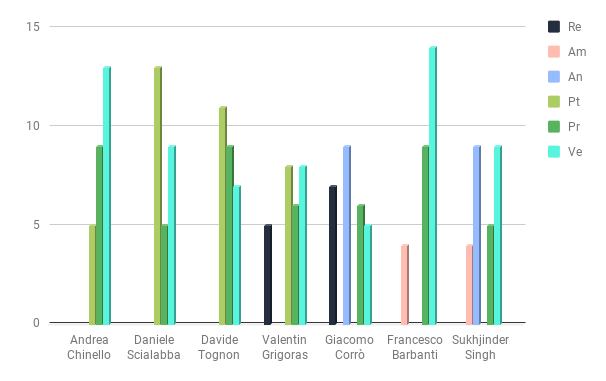
\includegraphics[scale=0.6]{immagini/pa_isto.png}
            \caption{Istogramma della distribuzione delle ore per ruolo in fase di progettazione architetturale}
        \end{figure}

        \subsubsection{Prospetto economico}
        Le ore e i costi dei vari ruoli di questa fase sono i seguenti:
        \begin{table}[H]
            
            \centering
            \renewcommand{\arraystretch}{2.6}
            \rowcolors{3}{tableRow}{}
            \begin{tabular}{c c c}
                \rowcolor[HTML]{232f3e} 
                \multicolumn{1}{c}{\color[HTML]{FFFFFF} \textbf{Ruolo}} &
                \multicolumn{1}{c}{\color[HTML]{FFFFFF} \textbf{Ore}} &
                \multicolumn{1}{c}{\color[HTML]{FFFFFF} \textbf{Costo}} \\
                \roleProjectManager&12&360\\
                \roleAdministrator&8&160\\
                \roleAnalyst&18&450\\
                \roleDesigner&37&814\\
                \roleProgrammer&49&735\\
                \roleVerifier&65&975\\
                \textbf{Totale}&\textbf{189}&\textbf{3494,00 \euro}\\
            \end{tabular}
            \caption {Ore e costo per ruolo durante la fase di progettazione architetturale} \label{table:Prospetto economico tabella}
        \end{table}

        \pagebreak

        La suddivisione dei ruoli è così raffigurabile:
        \begin{figure}[H]
            \centering
            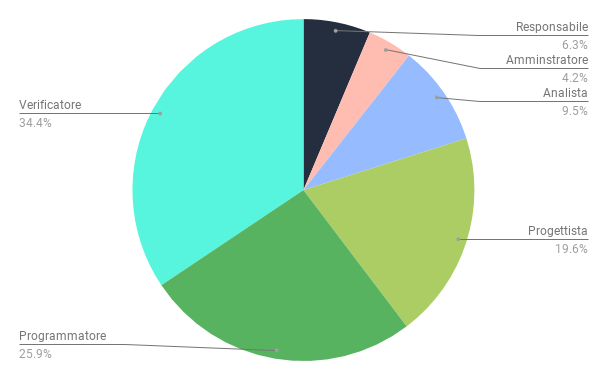
\includegraphics[scale=0.6]{immagini/pa_pie.png}
            \caption{Aerogramma della distribuzione delle ore per ruolo in fase di progettazione architetturale}
        \end{figure}

    \subsection{Fase di progettazione di dettaglio e codifica}
        \subsubsection{Prospetto orario}
        La distribuzione delle ore in questa fase è riassunta nella seguente tabella:
            \begin{table}[H]
                
                \centering
                \renewcommand{\arraystretch}{2.6}
                \rowcolors{3}{tableRow}{}
                \begin{tabular}{c c c c c c c c}
                    \rowcolor[HTML]{232f3e} 
                    \multicolumn{1}{c}{\color[HTML]{FFFFFF} \textbf{Nominativo}} &
                    \multicolumn{1}{c}{\color[HTML]{FFFFFF} \textbf{Re}} &
                    \multicolumn{1}{c}{\color[HTML]{FFFFFF} \textbf{Am}} &
                    \multicolumn{1}{c}{\color[HTML]{FFFFFF} \textbf{An}} &
                    \multicolumn{1}{c}{\color[HTML]{FFFFFF} \textbf{Pt}} &
                    \multicolumn{1}{c}{\color[HTML]{FFFFFF} \textbf{Pr}} &
                    \multicolumn{1}{c}{\color[HTML]{FFFFFF} \textbf{Ve}} &
                    \multicolumn{1}{c}{\color[HTML]{FFFFFF} \textbf{Totale}} \\
                    \andrea &-&-&22&-&18&15&55\\
                    \daniele &-&8&-&27&-&20&55\\
                    \davide &9&-&-&24&22&-&55\\
                    \valentin &9&-&-&24&22&-&55\\
                    \giacomo &-&-&-&22&16&17&55\\ 
                    \francesco &-&-&-&20&15&20&55\\ 
                    \singh &9&-&-&24&22&-&55\\
                \end{tabular}
                \caption {Distribuzione di ore nella fase di Progettazione di dettaglio e codifica} \label{table:Suddivisione ruoli in ore}
            \end{table} 
            
            \pagebreak
            
            È possibile raffigurare l'allocazione dei ruoli nel seguente istogramma:
            \begin{figure}[H]
                \centering
                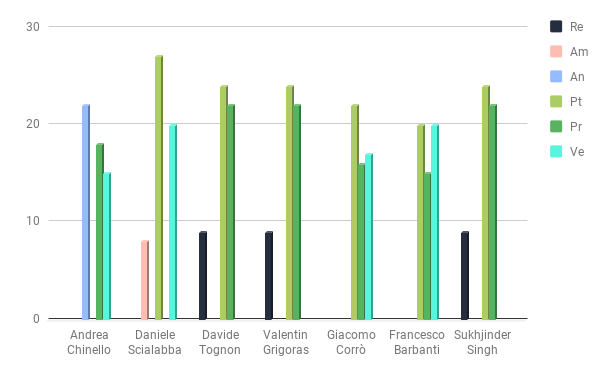
\includegraphics[scale=0.6]{immagini/pdc_isto.png}
                \caption{Istogramma della distribuzione delle ore per ruolo in fase di progettazione dettaglio e codifica}
            \end{figure}

        \subsubsection{Prospetto economico}
        Le ore e i costi dei vari ruoli di questa fase sono i seguenti:
            \begin{table}[H]
                
                \centering
                \renewcommand{\arraystretch}{2.6}
                \rowcolors{3}{tableRow}{}
                \begin{tabular}{c c c}
                    \rowcolor[HTML]{232f3e} 
                    \multicolumn{1}{c}{\color[HTML]{FFFFFF} \textbf{Ruolo}} &
                    \multicolumn{1}{c}{\color[HTML]{FFFFFF} \textbf{Ore}} &
                    \multicolumn{1}{c}{\color[HTML]{FFFFFF} \textbf{Costo}} \\
                    \roleProjectManager&27&810,00 \euro\\
                    \roleAdministrator&8&160,00 \euro\\
                    \roleAnalyst&22&550,00 \euro\\
                    \roleDesigner&141&3102,00 \euro\\
                    \roleProgrammer&115&1725,00 \euro\\
                    \roleVerifier&72&1080,00 \euro\\
                    \textbf{Totale}&\textbf{385}&\textbf{7427,00 \euro}\\
                \end{tabular}
                \caption {Ore e costo per ruolo durante la fase di progettazione dettaglio e codifica} \label{table:Prospetto economico tabella}
            \end{table} 
            
            \pagebreak

            La suddivisione dei ruoli è raffigurabile nel seguente grafico:
            \begin{figure}[H]
                \centering
                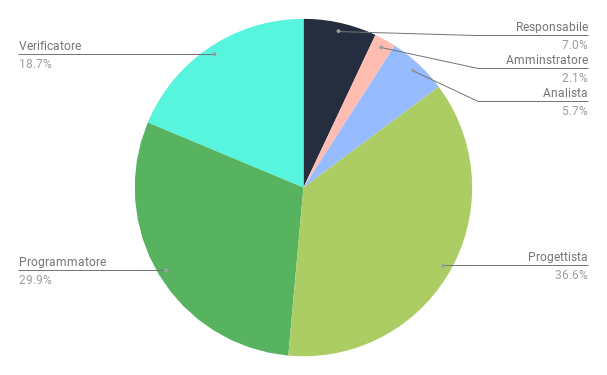
\includegraphics[scale=0.6]{immagini/pdc_pie.png}
                \caption{Aerogramma della distribuzione delle ore per ruolo in fase di progettazione dettaglio e codifica}
            \end{figure}

    \subsection{Fase di validazione e collaudo}
        \subsubsection{Prospetto orario}
        La distribuzione oraria di questa fase è la seguente:
            \begin{table}[H]
                
                \centering
                \renewcommand{\arraystretch}{2.6}
                \rowcolors{3}{tableRow}{}
                \begin{tabular}{c c c c c c c c}
                    \rowcolor[HTML]{232f3e} 
                    \multicolumn{1}{c}{\color[HTML]{FFFFFF} \textbf{Nominativo}} &
                    \multicolumn{1}{c}{\color[HTML]{FFFFFF} \textbf{Re}} &
                    \multicolumn{1}{c}{\color[HTML]{FFFFFF} \textbf{Am}} &
                    \multicolumn{1}{c}{\color[HTML]{FFFFFF} \textbf{An}} &
                    \multicolumn{1}{c}{\color[HTML]{FFFFFF} \textbf{Pt}} &
                    \multicolumn{1}{c}{\color[HTML]{FFFFFF} \textbf{Pr}} &
                    \multicolumn{1}{c}{\color[HTML]{FFFFFF} \textbf{Ve}} &
                    \multicolumn{1}{c}{\color[HTML]{FFFFFF} \textbf{Totale}} \\
                    \andrea &8&-&-&3&6&3&20\\
                    \daniele &-&8&-&-&6&6&20\\
                    \davide &-&5&-&-&7&8&20\\
                    \valentin &-&5&-&-&7&8&20\\
                    \giacomo &-&-&-&-&10&10&20\\ 
                    \francesco &-&-&-&-&10&10&20\\ 
                    \singh &-&-&-&-&10&10&20\\
                \end{tabular}
                \caption {Distribuzione di ore nella fase di Validazione e collaudo} \label{table:Suddivisione ruoli in ore}
            \end{table} 
            
            \pagebreak

            È possibile raffigurare l'allocazione dei ruoli nel seguente istogramma:
            \begin{figure}[H]
                \centering
                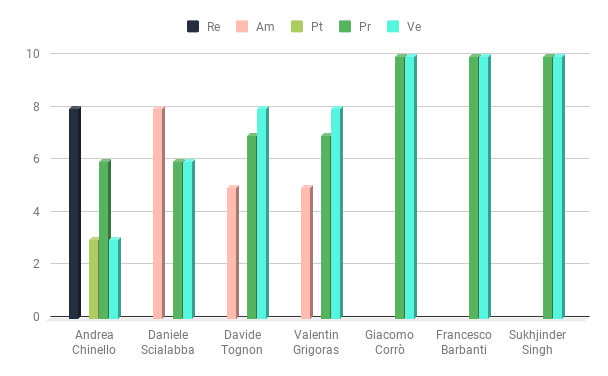
\includegraphics[scale=0.6]{immagini/vc_isto.png}
                \caption{Istogramma della distribuzione delle ore per ruolo in fase di progettazione architetturale}
            \end{figure}
    
        \subsubsection{Prospetto economico}
        Le ore e i costi dei vari ruoli di questa fase sono i seguenti:
            \begin{table}[H]
                
                \centering
                \renewcommand{\arraystretch}{2.6}
                \rowcolors{3}{tableRow}{}
                \begin{tabular}{c c c}
                    \rowcolor[HTML]{232f3e} 
                    \multicolumn{1}{c}{\color[HTML]{FFFFFF} \textbf{Ruolo}} &
                    \multicolumn{1}{c}{\color[HTML]{FFFFFF} \textbf{Ore}} &
                    \multicolumn{1}{c}{\color[HTML]{FFFFFF} \textbf{Costo}} \\
                    \roleProjectManager&8&240,00 \euro\\
                    \roleAdministrator&18&360,00 \euro\\
                    \roleAnalyst&0&0\\
                    \roleDesigner&3&66,00 \euro\\
                    \roleProgrammer&56&840,00 \euro\\
                    \roleVerifier&55&825,00 \euro\\
                    \textbf{Totale}&\textbf{140}&\textbf{2331,00 \euro}\\
                \end{tabular}
                \caption {Ore e costo per ruolo durante la fase di validazione e collaudo} \label{table:Prospetto economico tabella}
            \end{table} 
            
            \pagebreak

        La suddivisione dei ruoli è raffigurabile nel seguente grafico:
            \begin{figure}[H]
                \centering
                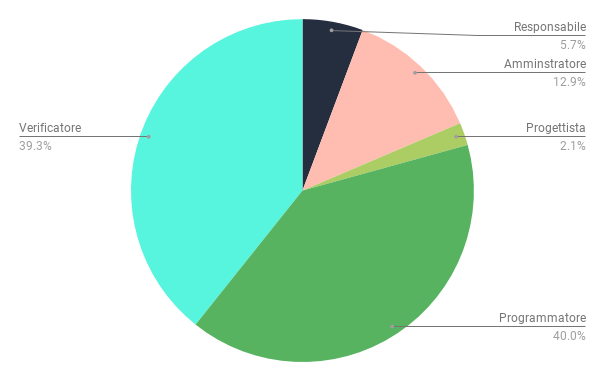
\includegraphics[scale=0.6]{immagini/vc_pie.png}
                \caption{Aerogramma della distribuzione delle ore per ruolo in fase di Validazione e collaudo}
            \end{figure}
    
    \subsection{Totale ore investite}
        \subsubsection{Prospetto orario}
        Di seguito vengono riportate il totale delle ore per il progetto dato dalla somma delle ore di investimento e di ore rendicontate:
            \begin{table}[H]
                
                \centering
                \renewcommand{\arraystretch}{2.6}
                \rowcolors{3}{tableRow}{}
                \begin{tabular}{c c c c c c c c}
                    \rowcolor[HTML]{232f3e} 
                    \multicolumn{1}{c}{\color[HTML]{FFFFFF} \textbf{Nominativo}} &
                    \multicolumn{1}{c}{\color[HTML]{FFFFFF} \textbf{Re}} &
                    \multicolumn{1}{c}{\color[HTML]{FFFFFF} \textbf{Am}} &
                    \multicolumn{1}{c}{\color[HTML]{FFFFFF} \textbf{An}} &
                    \multicolumn{1}{c}{\color[HTML]{FFFFFF} \textbf{Pt}} &
                    \multicolumn{1}{c}{\color[HTML]{FFFFFF} \textbf{Pr}} &
                    \multicolumn{1}{c}{\color[HTML]{FFFFFF} \textbf{Ve}} &
                    \multicolumn{1}{c}{\color[HTML]{FFFFFF} \textbf{Totale}} \\
                    \andrea &16&5&34&8&33&31&127\\
                    \daniele &5&26&5&40&11&40&127\\
                    \davide &9&5&4&41&38&30&127\\
                    \valentin &19&5&6&38&35&24&127\\
                    \giacomo &7&5&24&27&32&32&127\\ 
                    \francesco &5&4&15&20&34&49&127\\ 
                    \singh &9&9&24&24&37&24&127\\
                \end{tabular}
                \caption {Distribuzione oraria totale delle ore investite e rendicontate} \label{table:Suddivisione ruoli in ore totali}
            \end{table} 
            
            \pagebreak

            Il seguente istogramma rappresenta la suddivisione oraria:
            \begin{figure}[H]
                \centering
                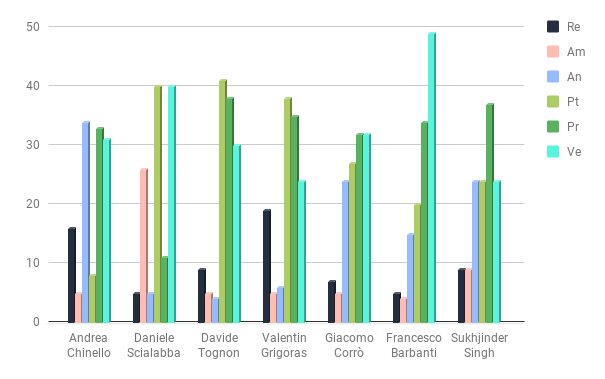
\includegraphics[scale=0.6]{immagini/ore_totali_isto.png}
                \caption{Istogramma della distribuzione delle ore investite e rendicontate}
            \end{figure}
            
            \subsubsection{Prospetto economico}
            Le ore e i costi dei vari ruoli sono i seguenti:
                \begin{table}[H]
                    
                    \centering
                    \renewcommand{\arraystretch}{2.6}
                    \rowcolors{3}{tableRow}{}
                    \begin{tabular}{c c c}
                        \rowcolor[HTML]{232f3e} 
                        \multicolumn{1}{c}{\color[HTML]{FFFFFF} \textbf{Ruolo}} &
                        \multicolumn{1}{c}{\color[HTML]{FFFFFF} \textbf{Ore}} &
                        \multicolumn{1}{c}{\color[HTML]{FFFFFF} \textbf{Costo}} \\
                        \roleProjectManager&70&2100,00 \euro\\
                        \roleAdministrator&59&1180,00 \euro\\
                        \roleAnalyst&112&2800,00 \euro\\
                        \roleDesigner&198&4356,00 \euro\\
                        \roleProgrammer&220&3300,00 \euro\\
                        \roleVerifier&230&3450,00 \euro\\
                        \textbf{Totale}&\textbf{889}&\textbf{17186,00 \euro}\\
                    \end{tabular}
                    \caption {Prospetto dei costi delle ore investite e rendicontate}
                \end{table} 
                
                \pagebreak

            La suddivisione dei ruoli è raffigurabile nel seguente grafico:
                \begin{figure}[H]
                    \centering
                    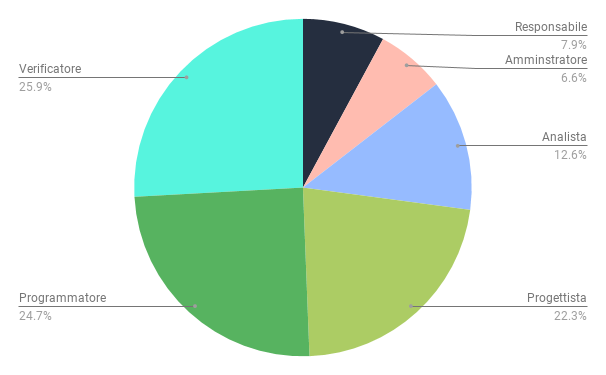
\includegraphics[scale=0.6]{immagini/ore_totali_pie.png}
                    \caption{Aerogramma delle ore investite e rendicontate per ruolo}
                \end{figure}


    \subsection{Totale ore rendicontate}
        \subsubsection{Prospetto orario}
        Nel seguito sono riportate le ore rendicontate nel preventivo a carico del committente:
            \begin{table}[H]
                
                \centering
                \renewcommand{\arraystretch}{2.6}
                \rowcolors{3}{tableRow}{}
                \begin{tabular}{c c c c c c c c}
                    \rowcolor[HTML]{232f3e} 
                    \multicolumn{1}{c}{\color[HTML]{FFFFFF} \textbf{Nominativo}} &
                    \multicolumn{1}{c}{\color[HTML]{FFFFFF} \textbf{Re}} &
                    \multicolumn{1}{c}{\color[HTML]{FFFFFF} \textbf{Am}} &
                    \multicolumn{1}{c}{\color[HTML]{FFFFFF} \textbf{An}} &
                    \multicolumn{1}{c}{\color[HTML]{FFFFFF} \textbf{Pt}} &
                    \multicolumn{1}{c}{\color[HTML]{FFFFFF} \textbf{Pr}} &
                    \multicolumn{1}{c}{\color[HTML]{FFFFFF} \textbf{Ve}} &
                    \multicolumn{1}{c}{\color[HTML]{FFFFFF} \textbf{Totale}} \\
                    \andrea &8&-&22&8&33&31&102\\
                    \daniele &-&16&-&40&11&35&102\\
                    \davide &9&5&-&35&38&15&102\\
                    \valentin &14&5&-&32&35&16&102\\
                    \giacomo &7&-&9&22&32&32&102\\ 
                    \francesco &-&4&-&20&34&44&102\\ 
                    \singh &9&4&9&24&37&19&102\\
                \end{tabular}
                \caption {Distribuzione oraria totale delle ore rendicontate} \label{table:Suddivisione ruoli in ore rendicontate}
            \end{table} 
            
            \pagebreak

            Il seguente istogramma rappresenta la suddivisione oraria:
            \begin{figure}[H]
                \centering
                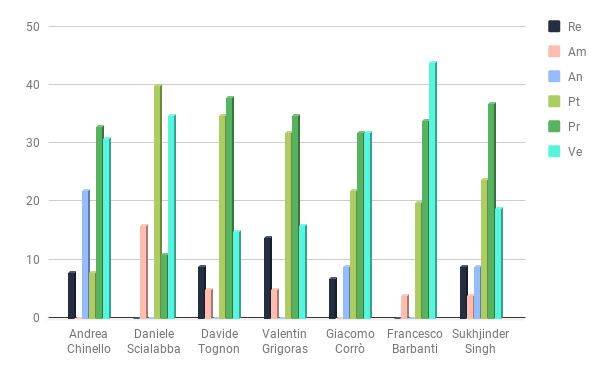
\includegraphics[scale=0.6]{immagini/ore_rendicontate_isto.png}
                \caption{Istogramma della distribuzione delle ore rendicontate}
            \end{figure}

        \subsubsection{Prospetto economico}
        Le ore e i costi dei vari ruoli sono i seguenti:
            \begin{table}[H]
                
                \centering
                \renewcommand{\arraystretch}{2.6}
                \rowcolors{3}{tableRow}{}
                \begin{tabular}{c c c}
                    \rowcolor[HTML]{232f3e} 
                    \multicolumn{1}{c}{\color[HTML]{FFFFFF} \textbf{Ruolo}} &
                    \multicolumn{1}{c}{\color[HTML]{FFFFFF} \textbf{Ore}} &
                    \multicolumn{1}{c}{\color[HTML]{FFFFFF} \textbf{Costo}} \\
                    \roleProjectManager&47&1410,00 \euro\\
                    \roleAdministrator&34&680,00 \euro\\
                    \roleAnalyst&40&1000,00 \euro\\
                    \roleDesigner&181&3982,00 \euro\\
                    \roleProgrammer&220&3300,00 \euro\\
                    \roleVerifier&192&2880,00 \euro\\
                    \textbf{Totale}&\textbf{714}&{13252,00 \euro}\\
                \end{tabular}
                \caption {Prospetto dei costi delle ore rendicontate}
            \end{table} 
            
            \pagebreak

        La suddivisione dei ruoli è raffigurabile nel seguente grafico:
            \begin{figure}[H]
                \centering
                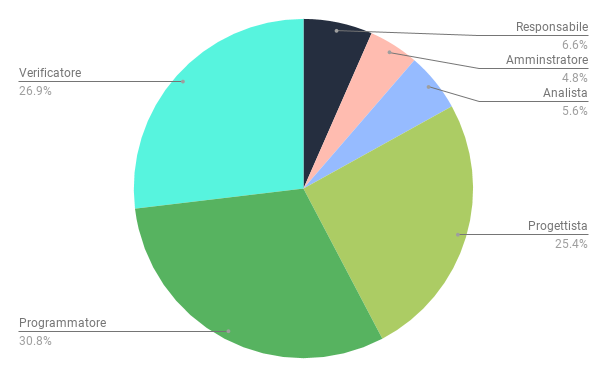
\includegraphics[scale=0.6]{immagini/ore_rendicontate_pie.png}
                \caption{Aerogramma delle ore rendicontate per ruolo}
            \end{figure}

        \subsubsection{Conclusioni}Il totale del preventivo per il progetto è di 13252,00 \euro.